\documentclass{article}
\usepackage{graphicx}

\begin{document}

\title{6.854 Final Project}
\author{Arsen Mamikonyan; Hayk Saribekyan}


\maketitle

\begin{abstract}
    In this paper we review and implement two algorithms presented by Bokal et al.\cite{bokal_et_al:LIPIcs:2015:5113}, and Chan and Pratt \cite{chan_et_al:LIPIcs:2016:5920}, presented in SoCG'15 and SoCG'16 respectively. Both works introduce novel approaches to finding maximal subsequences with given hereditary properties.
\end{abstract}

\section{Introduction}

With increasing number of sensors and location-tracking devices, there are massive datasets describing movements of people, animals, robots, etc. Since the datasets mostly describe trajectories of movement, often each location point is associated with a timestamp. As a result, in the process of analysing such datasets, efficient algorithms for time range queries are required.

This paper discusses problems of the following nature: given a sequence of points $S = s_1, \dots, s_n$, and a property $P$ defined on a sequence of points. For any given range $[i, j]$, we want to answer whether $P$ is true for $s_i, \dots, s_j$. Additionally, we restrict $P$ to be a hereditary property i.e. if $P$ holds for sequence set $A$, then $P$ also holds for any subsequence of $A$. The ability to answer these queries has practical applications and, in particular, it is the case for the two problems discussed in this paper.

Suppose we have a data structure that for any index $i$ retrieves the largest integer $j^*(i)$ such that $P$ is true for the sequence $S[i, j^*(i)]$. Then, it is trivial to check whether $P$ holds for $S[i, j]$ as one only needs to compare $j$ and $j^*(i)$. Therefore, the time range query problem reduces to building such data structure. Each of the two papers reviewed here present a general framework that can be used to build such data structures for a variety of problems.

\cite{bokal_et_al:LIPIcs:2015:5113,chan_et_al:LIPIcs:2016:5920} use their frameworks to efficiently solve the range query problem for different properties $P$. We have implemented one algorithm from each paper. The first one is the \textit{monotonicity} property. A sequence of points $S$ in two-dimensional space is monotone if there is a line $l$, for which if points of $S$ are projected on $l$, their order is maintained. The algorithm described in \cite{bokal_et_al:LIPIcs:2015:5113} is linear. The second one is the \textit{clustering} property. We will call a set of points $S$ clustered, if the largest distance between any pair of them (the diameter of $S$) is at most 1. \cite{chan_et_al:LIPIcs:2016:5920} present a $O(n\log n)$ algorithm to solve for this property.

For both of the problems there is a simple algorithm to solve them in quadratic time. We discovered that, while the algorithms presented in \cite{bokal_et_al:LIPIcs:2015:5113,chan_et_al:LIPIcs:2016:5920} are elegant and efficient, their implementation can be extremely complicated with many edge cases. Nevertheless, they are much faster for large enough datasets, thus, can be used in practice.

\section{Our contribution}
We've implemented
\begin{itemize}
\item In $O(n)$ time  we  can  find  all  maximal  subsequences  that  define  monotone  paths  in  some (subpath-dependent) direction. \cite{bokal_et_al:LIPIcs:2015:5113} 
\item In $O(n \log^2 n)$ time time we can find all maximal subsequences with diameter at most 1. \cite{chan_et_al:LIPIcs:2016:5920}
\end{itemize}

\section{Algorithms}
\subsection{$k^*$}

Let $k^*(i) = \inf_{m \geq i} \{d(i, m) > 1\}$. \textbf{Claim} $j^*(i-1) = \min(j^*(i), k^*(i-1))$. Thus after we calculate $k^*(i)$ for all elements, we can calculate $j^*(i)$ in $O(n)$ time by looping over all indices in the reverse order.

\subsection{Bokal et al Overview}
TODO: A page that deftly describes the algorithm we've implemented.

\subsection{Chan, Prat Overview}
TODO: A page that deftly describes the algorithm we've implemented.

\section{Implementation Details}
In this section we discuss some implementation details of the Chan, Pratt algorithm for diameter query problem. We skip the details of the monotonicity query, because it was relatively simple.

The novelty of the algorithm from Chan, Pratt is how they combine 1D range tree, with secondary structure that stores circle intersections. While the algorithm is elegant, its implementation is not. In particular, it is necessary to implement an intersection algorithm for arbitrary \textit{polyarcs}. A polyarc is a convex object, similar to a polygon, but instead of straight edges each side is an arc of a circle. The algorithm for the intersection of polyarcs is similar to that of polygons, however there are many more edge cases to consider.

\section{Experimental Results}

\subsection{Monotonicity}

TODO: Describe Naive algorithm which is a $O(n^2)$ algorithm.

\begin{figure}[!ht]
  \centering
  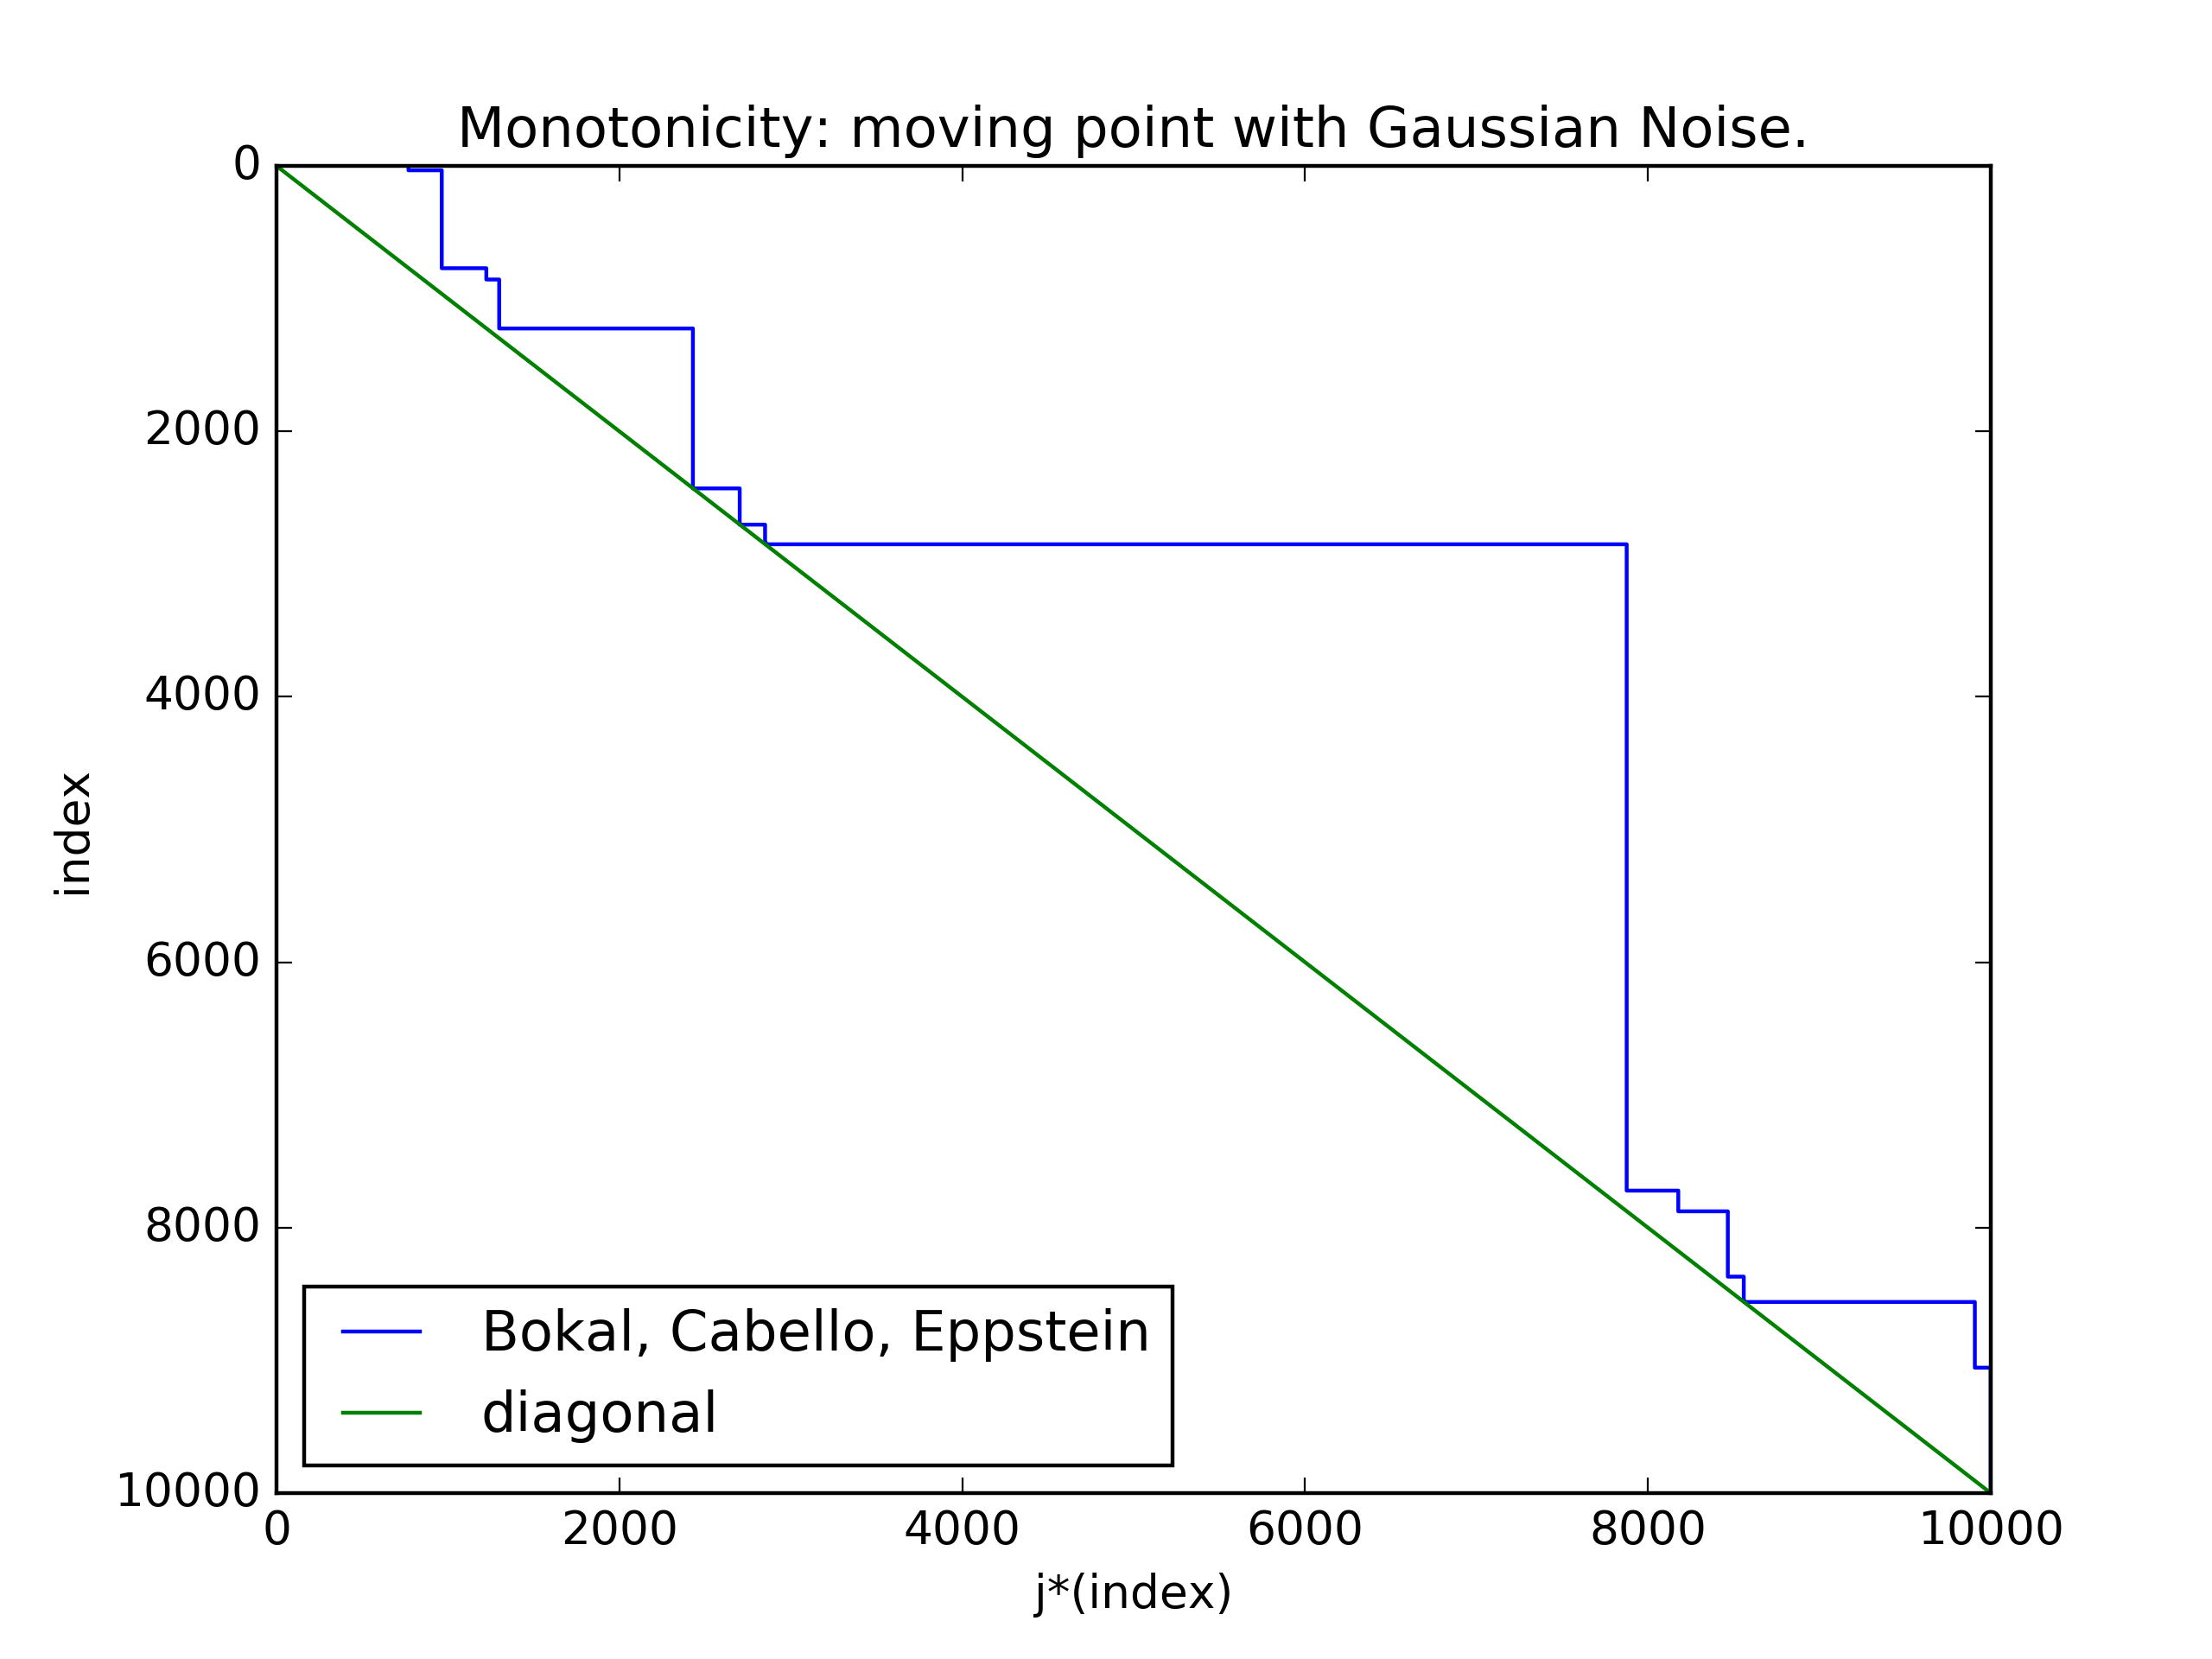
\includegraphics[height=8cm]{plots/monotonicity_moving_gaussian}
  \caption{Monotonicity algorithm results for moving point with Gaussian noise.}
  \label{fig:monotonicity_demo}
\end{figure}

First let's look at the monotonicity resutls. Here we use the following dataset.

We have a point moving along $x$ axis in the positive direction with speed 1 (i.e. 1 per index), we add Gaussian noise to this point to make the problem interseting. In Figure \ref{fig:monotonicity_demo} you can see results for noise with standard deviations $\sigma_y = 0.05, \sigma_y = 1$. After we generate the dataset, we run Bokal et. al algorithm on the dataset and the answer boundarries of the matrix $A$ that indicates if for points in range $[i, j]$ exists a common direction that has positive dot product with each of the displacements.

Figure \ref{fig:monotonicity_comparison} shows runtime differences in millliseonds between Naive algorithm and algorithm we presented from Bokal et al.
\begin{figure}[!ht]
  \centering
  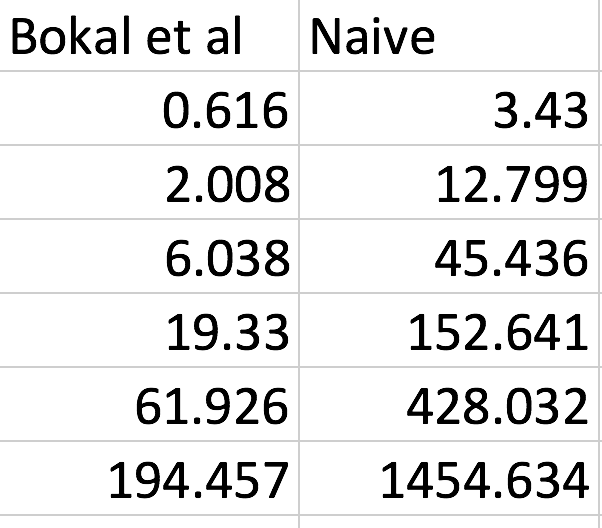
\includegraphics[height=5cm]{plots/monotonicity_comparison}
  \caption{Runtimes (in millseconds) of Naive and Bokal et. al}
  \label{fig:monotonicity_comparison}
\end{figure}

\subsection{Diameter}

Now the dataset is a random walk starting at the origin. At each step we uniform randomly pick a direction, and move 0.3 distance in that direction. We keep doing this until we have enough points for an experiment.

TODO: Describe Naive algorithm which is a $O(n^2)$ algorithm.

\begin{figure}[!h]
  \centering
  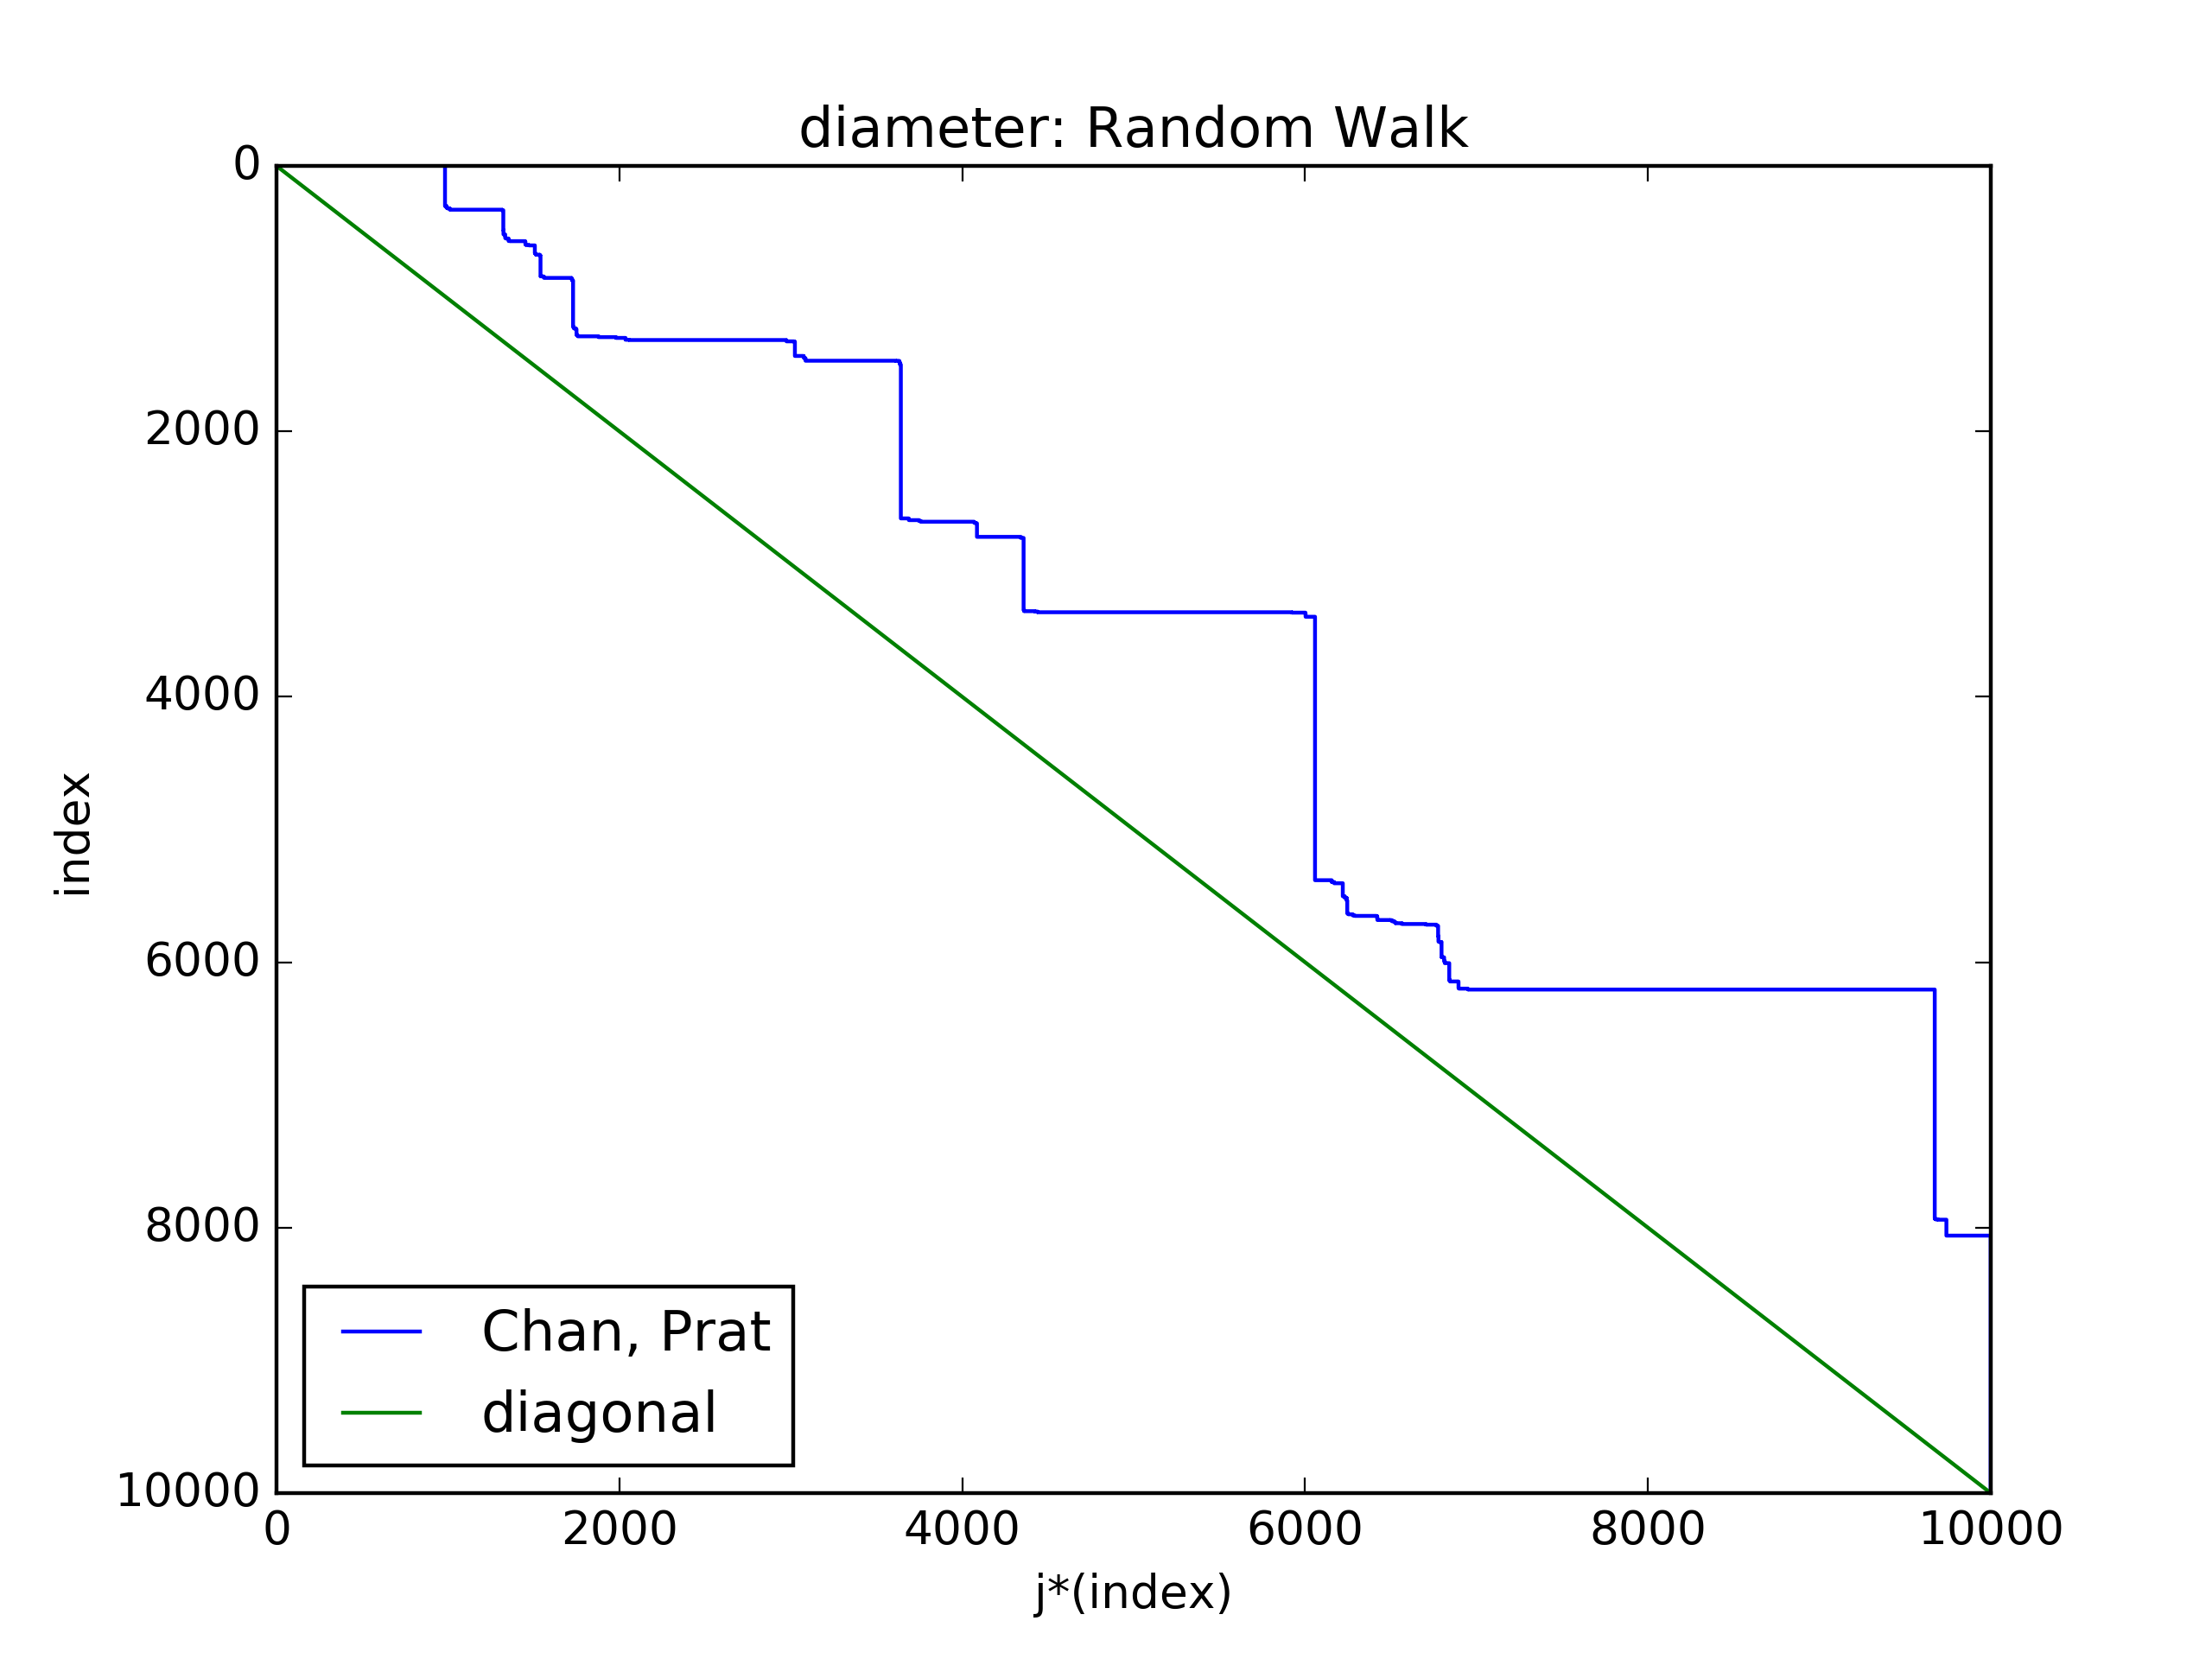
\includegraphics[height=8cm]{plots/diameter_random_walk}
  \caption{Caption...}
  \label{fig:diameter_demo}
\end{figure}

Figure \ref{fig:diameter_demo} shows boundaries of points that satisfy all points in range $[i, j]$ fall into some circle with radius 1.

Figure \ref{fig:diameter_comparison} will show results comparing runtimes of Naive algorithm with algorithm we presented from Bokal et al.
\begin{figure}[!ht]
  \centering
  
\includegraphics[height=5cm]{plots/diameter_comparison}
  \caption{Runtimes (in millseconds) of Naive and Chan, Prat [Similar to Figure \ref{fig:monotonicity_comparison}}
  \label{fig:diameter_comparison}
\end{figure}

\section{Conclusion}
It was really challanging to do an implementation project in computational geometry, some sentences in the papers take 100+ lines of code to implement. Thus, for small datasets, added complexity is not worth the speedup gained by the algorithm.

This was a great project otherwise, we've implemented couple of algorithms that we have seen during the lecture - sweep line, range tree, intersection of convex polygons using envelopes. Also couple that we had not found in Bokal et al and Chan, Prat.

\bibliographystyle{unsrt}
\bibliography{papers}
\end{document}
